\documentclass[aspectratio=169]{beamer}

% Custom theme and packages
\usepackage{beamertheme-custom}
% Custom symbols and commands
\usepackage{symbols-custom}

\graphicspath{{figures/}}

\author{Joachim Vandekerckhove}
\date{Spring 2025}

% Font
\usefonttheme[onlymath]{serif}

\title{An IRT analysis of a verbal aggression data set}

\begin{document}

\maketitle

\begin{frame}[fragile]{Verbal aggression}

By verbal aggression we mean verbal actions, such as cursing at oneself, scolding another person, or shouting\pause

While common, verbal aggression can be harmful\pause

Others see verbal aggression as a negative character trait\pause

Verbal aggression can cause mutual aggressive reactions and further escalation\pause

People differ in the degree to which they are able to inhibit their verbally aggressive impulses

\end{frame}


\begin{frame}[fragile]{Verbal aggression data set}

Collected at the University of Leuven, Belgium, by Kristof Vansteelandt\pause

Reported on in many publications, including \citeA{deboeck2004explanatory}\pause

Responses of 316 subjects (243 women and 73 men) to a questionnaire of 24 items, about verbal aggression\pause

Items describe a frustrating situation together with a possible verbal agression response

\end{frame}


\begin{frame}[fragile]{Verbal aggression data set}

The subset we will consider has 8 items.  Each item starts with one of the situations below:\\[2ex]

\bi \small\it
\item A bus fails to stop for me
\item I miss a train because a clerk gave me faulty information
\item The grocery store closes just as I am about to enter
\item The operator disconnects me when I had used up my last dime for a call
\ei\pause

\normalsize The item then continues either
\bi\small\it
\item I would want to curse
\item I would curse
\ei\pause

\normalsize
The corresponding item response is 1 if the respondent agrees with that sentence, and 0 if not

\end{frame}



\begin{frame}[fragile]{Formal description of the data subset}

Item-side variables
\bi
\item Scenario $\in \{1,2,3,4\}$
\item Behavior mode $\in \{\text{Do},\text{Want}\}$
\ei

Person-side variable
\bi
\item Gender: $\in \{\text{M},\text{F}\}$
\ei

Dependent variable
\bi
\item Response $\in \{0,1\}$
\ei

\end{frame}



\begin{frame}[fragile]{Research questions}
\bi
\item \emph{Item effect}: Do we see a difference between \textit{wanting} and \textit{doing}?
\item \emph{Person effect}: Do we see a gender difference in saying they would exhibit a verbally aggressive response?
\item \emph{Person-by-item interaction effect}: Do we see a gender difference in the difference between wanting and doing?
\ei\pause

In all these cases, we are interested in the probability that a respondent $p$ will answer `yes' on an item $i$.  In IRT, we investigate this response through the dominance parameter $\eta_{ip} = \theta_p - \beta_i$\pause

In the following analyses, we will look at systematic differences in $\theta$ and $\beta$\pause

A modern extension of the Rasch model considers more sophisticated views of the person and item parameters \cite{deboeck2004explanatory}
\end{frame}


\begin{frame}[fragile]{Explanatory item response models}

For example, the item parameter $\beta_i$ can be re-expressed as $\beta_i = \gamma \times W_i $:
$$ W_i =
\begin{cases}
1/2  & \text{if $i$ is want-item}\\
-1/2 & \text{if $i$ is do-item}
\end{cases}$$\pause
So that
$$ \beta_i = 
\begin{cases}
\gamma/2  & \text{if $i$ is want-item}\\
-\gamma/2 & \text{if $i$ is do-item}
\end{cases}$$\pause

We could then use this equation for the dominance: 
$$\eta_{ip} = \theta_p - \left(\gamma W_i\right)$$\pause
Now $\gamma$ is an effect size parameter -- it captures the difference in $\beta$ between the two kinds of items\pause

The rest of the model stays the same:
$P(X_{ip}=1) = \text{ilogit}(\eta_{ip})$

\end{frame}


\begin{frame}[fragile]{Explanatory item response models}

When we `decompose' parameters in this way -- replacing an item parameter $\beta_i$ by an expression like $\gamma W_i$ -- we call the resulting models \textit{explanatory}\pause

We say we have added a predictor ($W$) on the `item side' of the model\pause

This lets us say not only \emph{that} items differ in their difficulty, but also \emph{why}\\[3ex]\pause

\centering
\begin{tabular}{ccr}\hline
        \multicolumn{2}{c}{$\eta_{ip} = $ }&\\\cline{1-2}
  person part & item part & model type\\\hline
                   $\theta_p$ & $-\beta_i$ & doubly descriptive\\
    $\theta_p$ & $-\gamma W_i$ & item explanatory\\
 
\only<5->{$\alpha G_p + \epsilon_p$}  & 
\only<5->{$-\beta_i$} & 
\only<5->{person explanatory}\\
 
\only<6->{$\alpha G_p + \epsilon_p$} & 
\only<6->{$-\gamma W_i$}  &
\only<6->{doubly explanatory}\\
\multicolumn{2}{c}{\only<7->{$\alpha G_p + \epsilon_p-\gamma W_i-\delta W_iG_p$}}  &
\only<7->{interaction explanatory}\\\hline
\end{tabular}


\end{frame}


\begin{frame}[fragile]{Research questions}

	Do we see a difference between \textit{wanting} and \textit{doing}?   
	
	\hspace{.2in} $\rightarrow$ Need an item explanatory model\\[4ex]
	
	Do we see a gender difference in saying they would exhibit a verbally aggressive response?  
	
	\hspace{.2in} $\rightarrow$ Need a person explanatory model\\[4ex]
	
    Do we see a gender difference in the difference between wanting and doing? 

    \hspace{.2in} $\rightarrow$ Need an interaction explanatory model

\end{frame}


\begin{frame}[fragile]{Item-side question (\textit{wanting}, $W=\frac{1}{2}$, vs.\ \textit{doing}, $W=-\frac{1}{2}$)}\centering

$P\left(X_{ip}\right) = \text{ilogit}\left(\theta_p - \gamma W_i\right)$

\begin{table}[h]
	\scriptsize
	\label{tab:mCMCSummary}
	{
		\begin{tabular}{lrrrrr}
			\toprule
			\multicolumn{1}{c}{} & \multicolumn{3}{c}{Posterior} & \multicolumn{2}{c}{95\% Cred.\ Int.}\\
			\cline{2-4}\cline{5-6}
			Parameter & Mean & Median & SD & Lower & Upper  \\
			\cmidrule[0.4pt]{1-6}
			gamma & 0.385 & 0.383 & 0.163 & 0.064 & 0.706   \\
			\bottomrule
			% \addlinespace[1ex]
			% \multicolumn{9}{p{0.5\linewidth}}{\textit{Note.} The multivariate potential scale reduction factor is estimated at 1.001.} \\
		\end{tabular}
	}
\end{table}

\begin{figure}[htp]
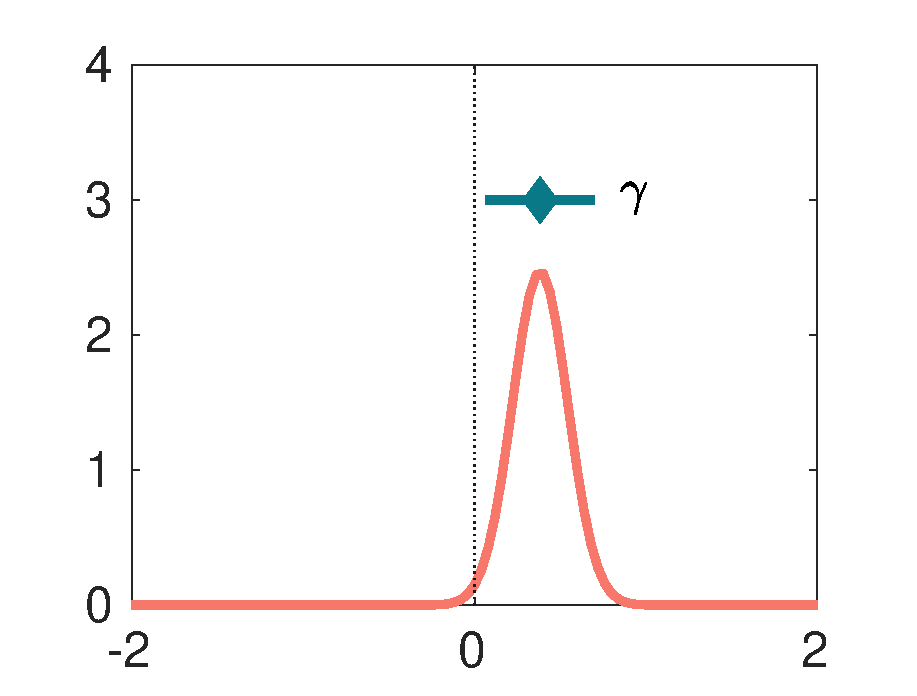
\includegraphics[scale=.3500]{ieirt}
\end{figure}

\end{frame}


\begin{frame}[fragile]{Person-side question (female, $G=-\frac{1}{2}$, vs.\ male, $G=\frac{1}{2}$)}\centering

$P\left(X_{ip}\right) = \text{ilogit}\left(\alpha G_p + \epsilon_p - \beta_i \right)$

\begin{table}[h]
	\scriptsize
	\label{tab:mCMCSummary}
	{
		\begin{tabular}{lrrrrr}
			\toprule
			\multicolumn{1}{c}{} & \multicolumn{3}{c}{Posterior} & \multicolumn{2}{c}{95\% Cred.\ Int.} \\
			\cline{2-4}\cline{5-6}
			Parameter & Mean & Median & SD & Lower & Upper   \\
			\cmidrule[0.4pt]{1-6}
			alpha & 0.542 & 0.536 & 0.342 & -0.116 & 1.228  \\
			\bottomrule
			% \addlinespace[1ex]
			% \multicolumn{9}{p{0.5\linewidth}}{\textit{Note.} The multivariate potential scale reduction factor is estimated at 1.000.} \\
		\end{tabular}
	}
\end{table}

\begin{figure}[htp]
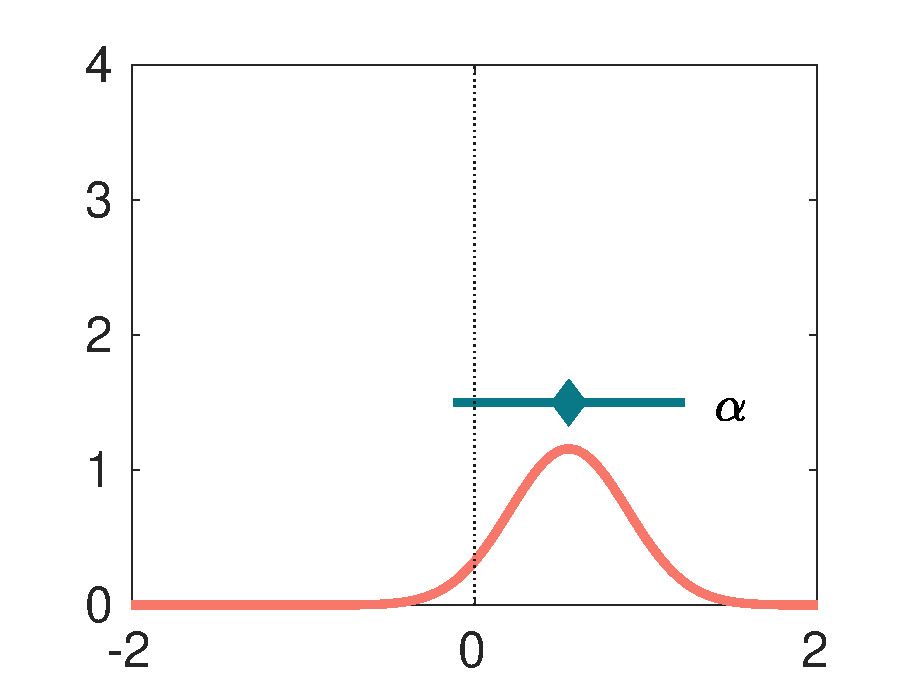
\includegraphics[scale=.3500]{peirt}
\end{figure}

\end{frame}


\begin{frame}[fragile]{Interaction question (gender $\times$ wanting vs.\ doing)}\centering

$P\left(X_{ip}\right) = \text{ilogit}\left(\alpha G_p + \epsilon_p - \gamma W_i - \delta G_p W_i\right)$

\begin{table}[h]
	\scriptsize
	\label{tab:mCMCSummary}
	{
		\begin{tabular}{lrrrrr}
			\toprule
			\multicolumn{1}{c}{} & \multicolumn{3}{c}{Posterior} & \multicolumn{2}{c}{95\% Cred.\ Int.}\\
			\cline{2-4}\cline{5-6}
			Parameter & Mean & Median & SD & Lower & Upper   \\
			\cmidrule[0.4pt]{1-6}
			alpha & 0.522 & 0.520 & 0.330 & -0.133 & 1.172  \\
			delta & -0.736 & -0.735 & 0.315 & -1.365 & -0.117  \\
			gamma & 0.365 & 0.365 & 0.166 & 0.035 & 0.692   \\
			\bottomrule
			% \addlinespace[1ex]
			% \multicolumn{9}{p{0.5\linewidth}}{\textit{Note.} The multivariate potential scale reduction factor is estimated at 1.003.} \\
		\end{tabular}
	}
\end{table}

\begin{figure}[htp]
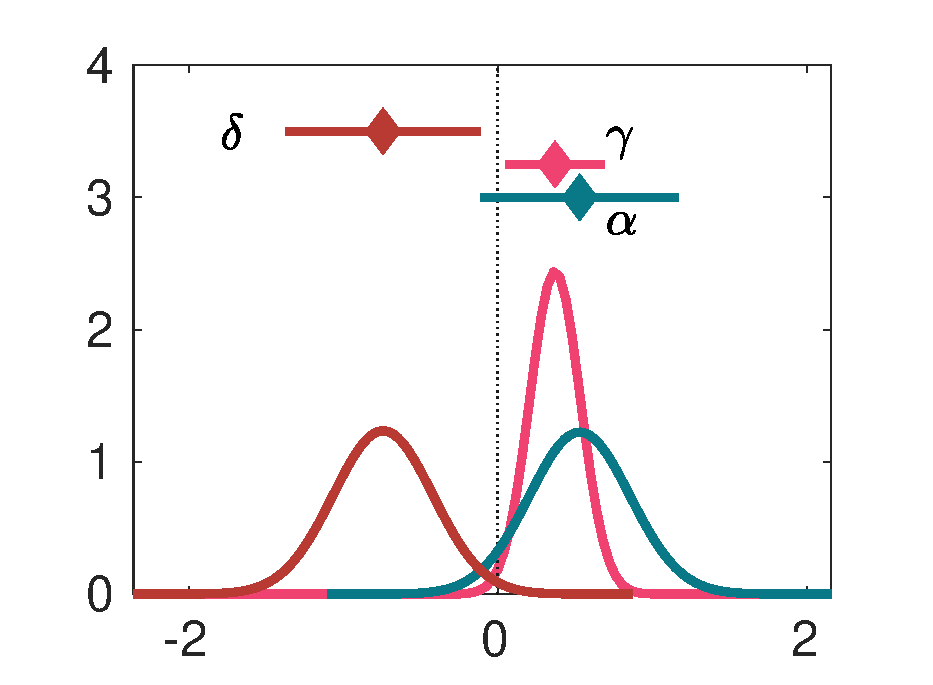
\includegraphics[scale=.3500]{deirt}
\end{figure}

\end{frame}


\begin{frame}[fragile]{Posterior predictive}
\begin{figure}[htp]
\centering
\includegraphics<1>[scale=.600]{irt_pp.eps}%
\includegraphics<2>[scale=.600]{irt_pp0.eps}%
\label{}
\end{figure}
\end{frame}


\begin{frame}[fragile]{Conclusions}

	Do we see a difference between \textit{wanting} and \textit{doing}?   
	
	\hspace{.2in} \only<2->{$\rightarrow$ Yes, wanting is more commonly selected than doing}\\[4ex]
	
	Do we see a gender difference in saying they would exhibit a verbally aggressive response?  
	
	\hspace{.2in} \only<3->{$\rightarrow$ We don't see a main effect}\\[4ex]
	
    Do we see a gender difference in the difference between wanting and doing? 

    \hspace{.2in} \only<4->{$\rightarrow$ Yes, the difference is smaller among male respondents}



\end{frame}


\begin{frame}[allowframebreaks]{References}
\bibliographystyle{apacite}
\bibliography{irt.bib}
\end{frame}



\maketitle



\begin{frame}[fragile]{Verbal aggression complete data set (part~1)}
\scriptsize
\begin{tabular}{ccccccccc}\hline
&&\multicolumn{2}{c}{Mode} & 
  \multicolumn{2}{c}{Blame} & 
  \multicolumn{3}{c}{Behavior}\\\cline{3-9}
Item & Situations &
Want & Do & Other &
Self & Curse & Scold & Shout\\\hline
 1 & S1 & 1 & 0 & 1 & 0 & 1 & 0 & 0 \\
 2 & S1 & 1 & 0 & 1 & 0 & 0 & 1 & 0 \\
 3 & S1 & 1 & 0 & 1 & 0 & 0 & 0 & 1 \\
 4 & S2 & 1 & 0 & 1 & 0 & 1 & 0 & 0 \\
 5 & S2 & 1 & 0 & 1 & 0 & 0 & 1 & 0 \\
 6 & S2 & 1 & 0 & 1 & 0 & 0 & 0 & 1 \\
 7 & S3 & 1 & 0 & 0 & 1 & 1 & 0 & 0 \\
 8 & S3 & 1 & 0 & 0 & 1 & 0 & 1 & 0 \\
 9 & S3 & 1 & 0 & 0 & 1 & 0 & 0 & 1 \\
10 & S4 & 1 & 0 & 0 & 1 & 1 & 0 & 0 \\
11 & S4 & 1 & 0 & 0 & 1 & 0 & 1 & 0 \\
12 & S4 & 1 & 0 & 0 & 1 & 0 & 0 & 1 \\\hline
\end{tabular}

\end{frame}

\begin{frame}[fragile]{Verbal aggression complete data set (part~2)}
\scriptsize
\begin{tabular}{ccccccccc}\hline
&&\multicolumn{2}{c}{Mode} & 
  \multicolumn{2}{c}{Blame} & 
  \multicolumn{3}{c}{Behavior}\\\cline{3-9}
Item & Situations &
Want & Do & Other &
Self & Curse & Scold & Shout\\\hline
13 & S1 & 0 & 1 & 1 & 0 & 1 & 0 & 0 \\
14 & S1 & 0 & 1 & 1 & 0 & 0 & 1 & 0 \\
15 & S1 & 0 & 1 & 1 & 0 & 0 & 0 & 1 \\
16 & S2 & 0 & 1 & 1 & 0 & 1 & 0 & 0 \\
17 & S2 & 0 & 1 & 1 & 0 & 0 & 1 & 0 \\
18 & S2 & 0 & 1 & 1 & 0 & 0 & 0 & 1 \\
19 & S3 & 0 & 1 & 0 & 1 & 1 & 0 & 0 \\
20 & S3 & 0 & 1 & 0 & 1 & 0 & 1 & 0 \\
21 & S3 & 0 & 1 & 0 & 1 & 0 & 0 & 1 \\
22 & S4 & 0 & 1 & 0 & 1 & 1 & 0 & 0 \\
23 & S4 & 0 & 1 & 0 & 1 & 0 & 1 & 0 \\
24 & S4 & 0 & 1 & 0 & 1 & 0 & 0 & 1 \\\hline
\end{tabular}

\end{frame}


\end{document}



